\documentclass[journal]{IEEEtran}
\usepackage{amsmath}
\usepackage{blindtext}
\usepackage{subcaption}
\usepackage{color}
\usepackage{graphicx}
\usepackage{mathtools}
\usepackage{algorithmicx}
\usepackage{algorithm}
\usepackage{color}
\newtheorem{theorem}{{\bf Theorem}}		% bf ka matlab bold letter mai likhna hota hai
\newtheorem{lemma}{{\bf Lemma}}
\newcommand{\vect}[1]{\boldsymbol{#1}}
\newcommand{\matx}[1]{\boldsymbol{#1}}
\begin{document}
	\title{Perfomance Analytic  Of Wireless System}
	\author{The Arun Sardar}
	\thanks{IIT GUWAHATI, D kumar is with company}
	\maketitle
	\begin{abstract}
		\blindtext
	\end{abstract}
\section{Introduction}
\blindtext
\subsection{Related Leiterature}
\blindtext
\subsection{focus}
\blindtext
section{System Mode}
\blindtext
\section{Analysis}
\blindtext
	\begin{equation}
		P_u = \left|h_{su}+h_{iu}\theta_{si}^{G_K}\right|^2
	\end{equation}
	\begin{equation}
		P_u\! =\!\left|h_{su}\!+\!h_{iu}\theta_{si}^{G_K}\right|^2
		\!\sigma^2\sigma^2\sigma^2\sigma^2\sigma^2\sigma^2\sigma^2\sigma^2\sigma^2
	\end{equation}
Inline equation
$x^a+b^c$.\blindtext
\begin{equation}
	Y = \left(x+\sum_{n=1}^Ny^n\right)
\end{equation}
the expression in~\eqref{eq:equation_try}
\begin{equation}
	Y = \left(x+\sum_{n_1=1}^{N_1}y^{{n_1}{n_2}}\right)
\end{equation}
\begin{align}		% agar equation no ko nahi dekhna chahta hai to {align*} likh do
	Y& = \left(x+\sum_{n_1=1}^{N_1}y^{{n_1}{n_2}}\right) \nonumber\\
	 & = \left(x+\sum_{n_1=1}^{N_1}D^{{n_1}{n_2}}\right)
\end{align}
\begin{multline}
		Y = \left(x+\sum_{n_1=1}^{N_1}y^{{n_1}{n_2}}\right)+b+b+b+b+b+b+b\\
		b+b+b+b+b+b\\ \\
		b+b+b+b+b+b\\ \\
		b+b+b+b+b+b\\ \\
		b+b+b+b+b+b\\ \\
	\end{multline}
\begin{equation}
	y=\frac{\splitfrac{a+b}{+c+d}}{\splitfrac{g+h}{+i+j}}
\end{equation}
\begin{figure*}
	\begin{equation*}
		Y = \left(x+\sum_{n=1}^Ny^n\right)..
	\end{equation*}
\noindent\rule{\textwidth}{0.5pt}
\end{figure*}
\begin{lemma}
	Hallo Lemma \cite{fenton2001fault}
\begin{IEEEproof}
	The proof is given in Appendix1~\ref{hh}
	\end{IEEEproof}
\end{lemma}
\begin{lemma}
	Hallo Lemma two
\begin{IEEEproof}
	The proof is given in Appendix1~\ref{hh}
\end{IEEEproof}
\end{lemma}
\begin{theorem}
	Hallo Theorem
\begin{IEEEproof}
	The proof is given in Appendix1~\ref{app:theorem_a}
\end{IEEEproof}
\end{theorem}
\begin{theorem}
	Hallo Theorem two
\begin{IEEEproof}
	The proof is given in Appendix1~\ref{hh}
\end{IEEEproof}
\end{theorem}
\blindtext
\begin{figure*}[!t]
	\centering
	\begin{subfigure}{0.4\textwidth}
		\centering
		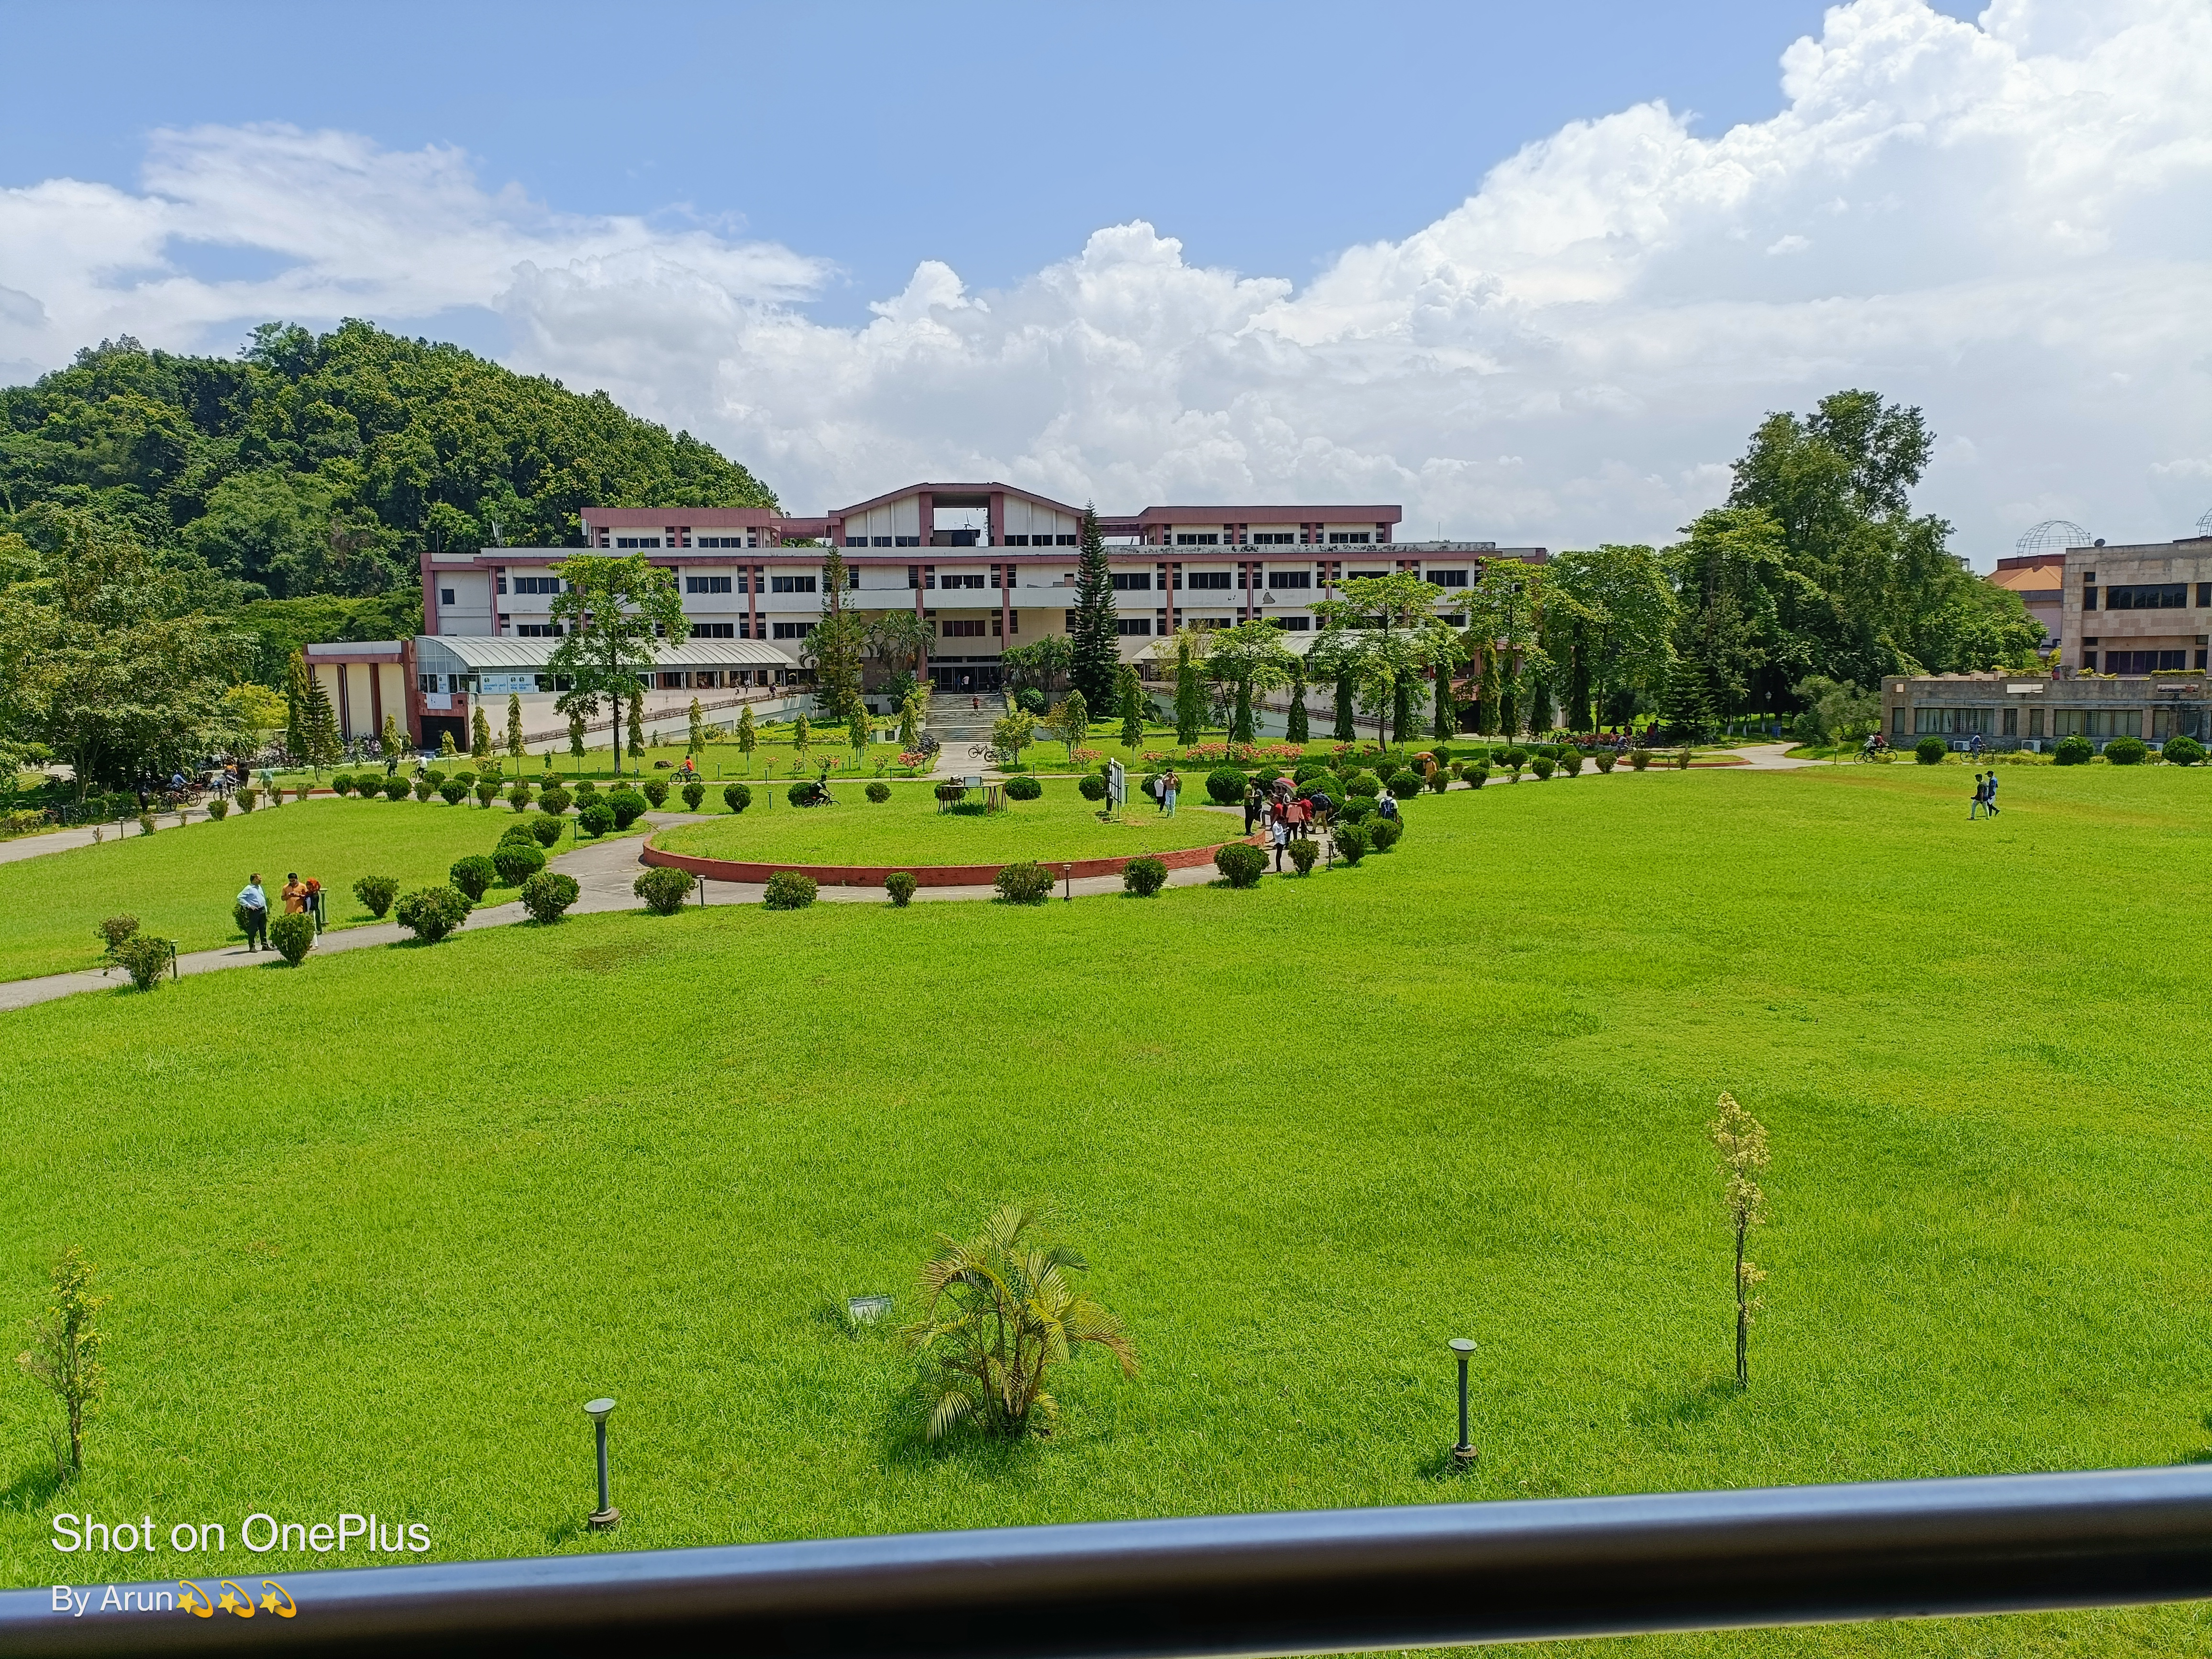
\includegraphics[width=1\linewidth]{iitg.jpg}
		\caption{Impact of $q$}
	\end{subfigure}
\begin{subfigure}{0.4\textwidth}
	\centering
	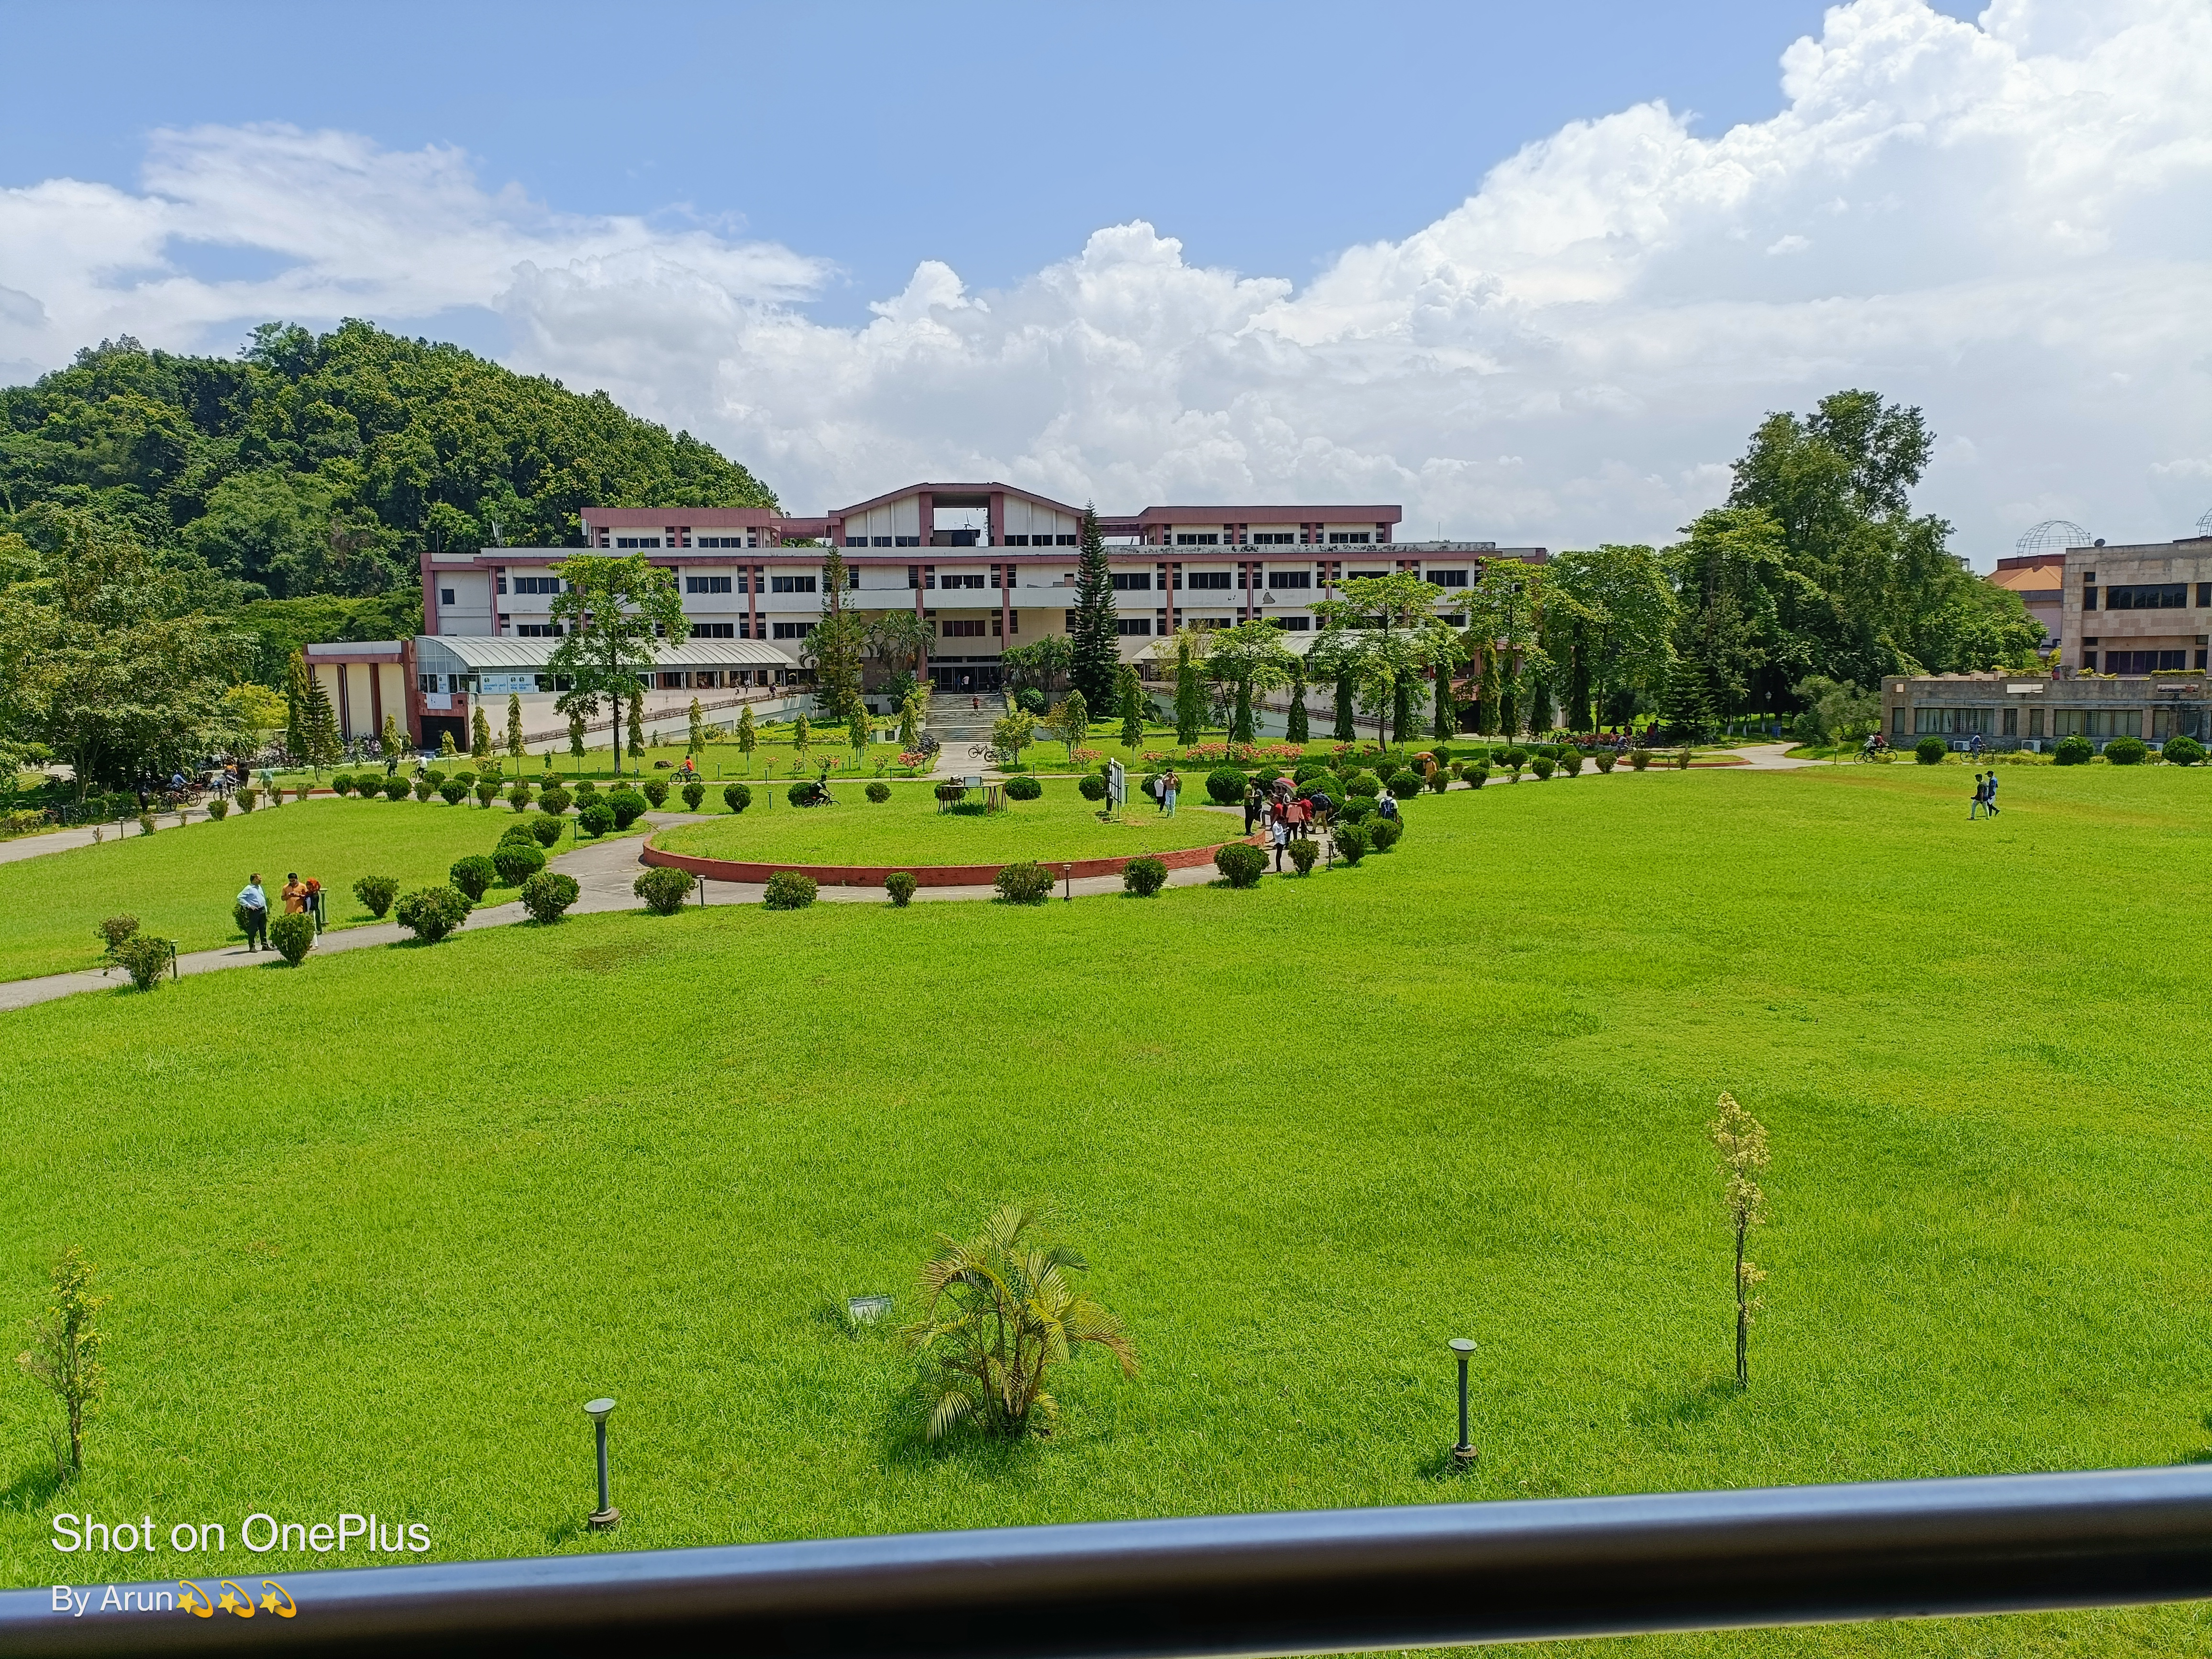
\includegraphics[width=1\linewidth]{iitg.jpg}
	\caption{Impact of $q$}
\end{subfigure}
\end{figure*}
\section{Conclusion}
\noindent this is our referance: \cite{fenton2001fault}
\blindtext
\appendices
\section{Proof of lemma~\ref{lem:lemma_w}}
\label{app:lemma_a}
\blindtext
\section{Proof of theorem~\ref{lem:lemma_w}}
\label{app:theorem_a}
\blindtext
\bibliographystyle{IEEEtran}
\bibliography{referance}

\end{document}